\documentclass{article}
\usepackage[utf8]{inputenc}
\usepackage{geometry}
\geometry{margin=1in}
\usepackage{amsmath}
\usepackage{amssymb}
\usepackage[ruled,vlined, linesnumbered]{algorithm2e}
\usepackage[english]{babel}
\usepackage[nottoc]{tocbibind}
\usepackage{xcolor}
\usepackage{natbib}
\usepackage{graphicx}
\usepackage{float}
\usepackage{hyperref}
\hypersetup{colorlinks=true, citecolor=black, linkcolor=., urlcolor=cyan}
\newtheorem{theorem}{Theorem}[section]
\bibliographystyle{ims}
% Custom commands / shortcuts
\providecommand{\sign}{\textrm{sign}}
\providecommand{\pb}[1]{\textcolor{red}{#1}}
\providecommand{\lam}{\lambda}

\title{Adaptive Hybrid Screening for Efficient Lasso Optimization}
\author{Chuyi Wang\\Department of Statistics and Actuarial Sciences\\University of Iowa
  \and
  Patrick Breheny\\Department of Biostatistics\\University of Iowa}
\date{}

\begin{document}

\maketitle

\begin{abstract}
Lasso type models are popular in statistics and machine learning, especially for variable selection in high-dimensional data. Typical practice is to tune the size of lasso penalty along a path of values. Due to modern data collection techniques, researchers need to analyse ultra high-dimension data with millions of features, which brings a great need for an efficient lasso optimization algorithm. Feature screening techniques have proven to be powerful for this need, because they can discard features and lead to a model with much less features. In this paper, we develop an adaptive hybrid screening framework where screening is carried out adpatively along the path of tuning parameter values. It reuses previous solutions in the path and reduces unhelpful heavy computations. It is a flexible framework that can be easily extended to different types of lasso models. Two applications for the standard lasso model and the sparse logistic model are shown as examples. We perform simulation study and real data study in a wide range of scenarios and the adaptive hybrid methods outperform other state-of-the-art method significantly and uniformly, with the greatest speedup in the most challenging scenarios.
\end{abstract}

\section{Introduction}

The least absolute shrinkage and selection operator, or lasso \citep{tibshirani1996regression}, is a popular model in statistics and machine learning, especially in high-dimensional problems. The model can be defined as the following modification of the least squares optimization problem:
\begin{equation}
  \label{eq:lasso}
  \hat{\beta}(\lambda)=\underset{\beta\in \mathbb{R}^p}{\mathrm{argmin}}\frac{1}{2n}||y-X\beta||_2^2+\lambda||\beta||_1,
\end{equation}
where $y$ is an $n\times 1$ vector of responses, $X=(x_1,x_2,...,x_p)$ is an $n\times p$ matrix of features, $\beta\in \mathbb{R}^p$ is the $p\times 1$ coefficient vector and $\lambda$ is the regularization tuning parameter. Throughout, we use $||\cdot||_2$ denotes the $l_2$ (Euclidean) norm and $||\cdot||_1$ denotes the $l_1$ norm. 

The lasso model has several attractive properties compared to least squares regression, including increased stability of estimation, increased prediction accuracy, and automatic variable selection arising from the fact that it yields sparse estimates of $\beta$.  As a result, it is widely applied in different fields, such as gene expression data analysis, image recognition and text mining, and has been extended in several ways, such as group lasso \citep{yuan2006model}, elastic net \citep{zou2005regularization} and sparse generalized linear models. Because of its wide popularity, solving the lasso efficiently is an important topic in statistics and machine learning.

Because the optimal value of $\lambda$ is not known in advance, typical practice is to solve for $\beta$ along a sequence of values of the tuning parameter $\lambda$, known as the solution path. While efficiently algorithms have been developed \citep{friedman2007pathwise} for the solution path, modern data collection and storage techniques allow researchers to measure an increasingly large number of features, which introduce additional computational challenges. In particular, it may not be possible to store the feature matrix, which can require many GBs of memory to store, in memory. One can resolve this problem by using a memory mapping package such as \textbf{bigmemory}, which allows us to store the feature matrix on disk and read it portions of it as needed; however, this results in frequent reading from disk, which is extremely slow compared to other parts of the algorithm and becomes a bottleneck with respect to the computational burden of fitting lasso models on very large data sets.

One promising technique to address this challenge is feature screening. The lasso model solution is sparse in the sense that most coefficients will be exactly zero; for these ``inactive'' coefficients we do not need their associated features.  In theory, if we knew which coefficients were nonzero at each value of $\lambda$, we could read into memory only those features and leave the remaining features on disk. In reality, we cannot know this prior to fitting the model -- however, through the clever use of feature screening rules, we can greatly reduce the number of times inactive features are read into memory, thereby minimizing the computational burden. There are many screening techniques where the solution obtained after screening will still be the global optimum given it exists, and in this paper we will only focus on this type of screening. In what follows, we refer to features left on disk as ``discarded'' features, although it is worth clarifying that this is not a permanent decision.  In particular, a feature can be discarded at one value of $\lambda$ but included in the list of potentially active features at other values of $\lambda$.

There are two important categories of feature screening rules: ``strong'' rules \citep{tibshirani2011regression, qian2019fast}, which occasionally incorrectly discard some active features, and ``safe'' rules \citep{ghaoui2010safe,wang2013lasso,xiang2012fast, xiang2011learning}, which are guaranteed never to do so.  As one might expect, strong rules tend to be easier to calculate; however, because mistakes are possible, one must add a post-convergence check to ensure that no features were incorrectly discarded. This check is not necessary with safe rules. However, safe rules are considerably less powerful at discarding features than strong rules. More recently, hybrid approaches \citep{Zeng2021} combining the two types of rules have been shown to be more efficient than either type of rule alone.

Safe screening rules can be implemented in one of two ways. Sequential rules do screening at each $\lambda$ value along the path using the previous solution as the reference, so they require heavy computation but are relatively powerful. One-step only use the solution at the beginning of the path as the reference. As a result, they require far less computational burden but they lose efficacy as the thus are faster but they cannot remain powerful along the path for long because they don't utilize previous solution.

In this paper, we propose an adaptive safe screening scheme. We begin choosing a solution as the reference for the safe rule and applying it to multiple solution steps along the path. However, unlike the one-step implementation, we monitor the power of the rule with this reference and once it is no longer effective, update the reference of the safe rule to the latest solution.  This process is repeated along the path, waiting until it is beneficial before investing in a new safe rule reference. This scheme avoids disadvantages of both sequential rules and one-step rules. Reusing the same solution as reference when the safe rule is still effective avoids unnecessary computations, while periodically updating the reference ensures that they maintain power across the entire path. We show that this adaptive approach can greatly reduce the computation time and outperforms other methods in all scenarios. Following the hybrid approaches, we also combined our approach with strong rules to form adaptive hybrid rules. Our method is general, and capable of utilizing any sequential safe rule, and thus readily extended to other lasso type models for which safe rules exist. Here, we illustrate its extensions to the logistic regression loss function and to the group lasso penalty.

This manuscript provides a brief review of existing feature screening rules in Section\ref{sec:existing} as well as the following novel contributions:

\begin{itemize}
    \item A new feature screening framework (Section 3.1,3.2), which updates the reference for screening along the grid of $\lambda$ values on any combination of strong screening rules and safe screening rules, which can generate a family of more efficient and scalable screening rules, compared to previous screening rules that are either sequential or one-step.
    \item Three specific applications of this framework, Ada-SSR-EDPP, Ada-SSR-Slores and Ada-SSR-EDPP for group lasso, for fitting lasso-penalized linear regression and logistic regression models, respectively (Section 3.4,4.1,4.2).
    \item An algorithm to determine when to update to a new reference $\lambda$ value for best efficiency (Section \ref{sec:adaptive}).
    \item Simulation studies (Section~\ref{sec:sim}) and real data analysis (Section~\ref{sec:real-data}) under a variety of scenarios, including testing data sets larger than memory, which showed that the proposed algorithms outperform other approaches in all cases, with substantial speed up.
    \item The Ada-SSR-SEDPP and Ada-SSR-Slores were implemented and added as new options to the publicly accessible \textbf{R} package \textbf{biglasso} \citep{zeng2017biglasso}, which was used to carry out the analyses in this manuscript.
\end{itemize}

\section{Existing feature screening rules}
\label{sec:existing}

Throughout this paper, it will be assumed that $y$ is centered and $\{x_j\}_{j=1}^p$ are centered and standardized:
\begin{equation}
  \label{eq:std}
  \sum_{i=1}^ny_i=0, \qquad \sum_{i=1}^n x_{ij}=0, \qquad \sum_{i=1}^n x_{ij}^2=n,\qquad j=1,2,...,p.
\end{equation}
Standardization ensures that the penalty is applied equally to all features, even if originally measured in different units. It also improves the efficiency and stability of the optimization, and helps to simplify optimization.  For example, under this standardization, the intercept is exactly 0 and thus may be ignored.  Standardization also simplifies the formulas for screening rules and thus allows for more efficient implementation.  Furthermore, this can be done without loss of generality as one can always obtain the solution on the original scale through a simple linear transformation of the standardized solution.

Typical practice when fitting lasso models is to solve for $\hat{\beta}(\lambda)$ along a decreasing sequence of $K+1$ values of $\lambda$: $\lambda_0 > \lambda_1 > \cdots > \lambda_K$.  As we will discuss shortly, we set $\lambda_0=\max_j|x_j^Ty/n|$ throughout; this ensures that $\hat{\beta}(\lambda_0)=0$, making it a natural point from which to start.

The goal of pathwise algorithms is to solve for this entire solution path.  This can be done efficiently by using ``warm starts'': using previous points on the path as initial values, as these are likely to be relatively close to the solution.  For the model at any $\lambda$-value $\lambda_{k+1}$, letting $r(\lambda_{k+1}) \equiv y-X\hat{\beta}(\lambda_{k+1})$ denote the vector of residuals, the solution $\hat{\beta}(\lambda_{k+1})$ can be computed using the previous solution $\hat{\beta}(\lambda_k)$ as the initial value in the algorithm. Pathwise coordinate descent is a algorithm that takes advantage of this idea and will be used as the lasso algorithm for the rest of the paper.

In convex optimization, the Karush-Kuhn-Tucker (KKT) conditions are both necessary and sufficient for any optimal solution.  Screening rules take advantage of these KKT conditions in order to discard inactive coefficients.  For the lasso, the KKT conditions governing the optimal solution $\hat{\beta}(\lambda)$ are given by
\begin{equation}
  \label{eq:kkt}
  \begin{aligned}
    x_j^Tr(\lambda)/n &= \lambda \, \sign \, \hat{\beta}_j(\lambda) & & \textrm{if } \hat{\beta}_j(\lambda)\neq 0,\\
    |x_j^Tr(\lambda)/n| &\leq \lambda & & \textrm{if } \hat{\beta}_j(\lambda)= 0.
  \end{aligned}
\end{equation}
If the residuals were known, we could safely conclude that $\hat{\beta}_j(\lambda)=0$ by verifying that the second condition holds as a strict inequality.  The complication, of course, is that the residuals are not known until after we have solved for all the coefficients.  However, when fitting a solution path, residuals at previous $\lambda$ values provide information about residuals at the next $\lambda$ value and thus may be used for screening. Note that if we have $\lambda_0=\max_j|x_j^Ty/n|$ and $\hat{\beta}(\lambda_0)=0$, then $r(\lambda_0)=y$ satisfies the KKT conditions and thus $\hat{\beta}(\lambda_0)=0$ is the optimal solution.

\subsection{Active-set Cycling}
\label{sec:active}

The simplest of all screening rules is to simply assume that features currently in the model will stay in the model and features currently excluded will remain excluded.  This is known as active-set cycling (AC) \citep{lee2007efficient}. It can be implemented on top of any lasso algorithm with no additional cost. When solving the coefficients for at $\lambda_{k+1}$, AC considers only features whose coefficients were non-zero at $\lambda_k$ and discards the other features. The lasso problem is then solved over this reduced number of coefficients.

After computing the solution, a post-convergence KKT conditions check is performed. Because the KKT conditions are sufficient for the solution to be optimal, if there is no violation, the solution to the smaller model will be exactly the same as if we solve the model with all features. If there are violations, corresponding features will be added to the model and this procedure is repeated. There are a finite number of features that can be added, so the procedure will end after finite repetitions. Because features enter the model relatively infrequently, typically only a small number of repetitions are needed, thereby providing a substantial speed up compared to solving the full lasso problem every time.

\subsection{Strong rules}

Each post-convergence check requires $O(np)$ operations and is therefore costly to repeat when violations occur.  These violations are inevitable in active-set cycling, as they occur every time a feature is added to the model.  Sequential strong rules (SSR) \citep{tibshirani2011regression} attempt to retain the basic idea of active-set cycling, but reduce violations by retaining features that are ``close'' to entering the model.

Given the solution $\hat{\beta}(\lambda_k)$ and residual vector $r(\lambda_k)=y-X\hat{\beta}(\lambda_k)$ at $\lambda_k$, the SSR discards the $j$-th feature at $\lambda_{k+1}$ if:
\begin{equation}
  \label{eq:ssr}
  |x_j^Tr(\lambda_k)/n|<2\lambda_{k+1}-\lambda_k.
\end{equation}
The SSR is derived from the KKT condition and the ``unit-slope'' assumption that the size of the slope of $x_j^Tr(\lambda)/n$ over $\lambda$ is bounded by 1. 

The biggest problem of SSR is that the ``unit-slope'' assumption may not hold and thus discarded features are not guaranteed to have zero coefficients. As with AC, a post-convergence KKT check is therefore needed for the discarded features to make sure their coefficients are truly zero. If violations occur, we again need to refit the model, adding the violating features and repeating the post-convergence check. Similar to the procedure in AC, there are a finite number of features that can be added, so the procedure will end after finite repetitions. Moreover, previous studies have shown that violations are rare, so the additional $O(np)$ cost for repeating a KKT check hardly ever arises.

SSR possesses the nice property that the quantity $x_j^Tr(\lambda_k)/n$ needed for SSR screening \eqref{eq:ssr} at $\lambda_{k+1}$ has already been calculated during post-convergence checking at $\lambda_k$ in \eqref{eq:kkt}. As this is the only computationally intensive aspect of SSR screening, and SSR violations are rare, its computational cost is roughly $O(npK)$.

\subsection{Safe rules}
\label{sec:safe}

Compared to strong rules, safe rules are never violated. Features can be discarded safely, with no need for post-covergence checking, as the coefficients are guaranteed to be zero by the rule. We will mainly focus on enhanced dual polytope projections (EDPP) rules\citep{wang2013lasso} because they outperform other known safe rules and are easy to incorporate into our method.

The EDPP rules are derived from the dual formulation of the lasso problem and provide a bound for the residual vector $r(\lambda)$. Then using the KKT conditions, some features can be guaranteed to have zero coefficients and be discarded safely. Two forms of the EDPP rule, basic EDPP (BEDPP) and sequential EDPP (SEDPP)\citep{wang2013lasso}, were proposed and under the standardization \eqref{eq:std} can be simplified in the following theorems \citep{Zeng2021}:

\begin{theorem}[BEDPP]
    For the lasso problem \eqref{eq:lasso}, let $\lambda_0:=\max_j|x_j^Ty/n|$ and $x_*=argmax_{x_j}|x_j^Ty/n|$. Under \eqref{eq:std} and for any $\lambda\in(0,\lambda_0]$, we have $\hat{\beta}_j(\lambda)=0$ if
    \begin{equation}
        \label{eq:bedpp}
        |(\lambda_0+\lambda)x_j^Ty-(\lambda_0-\lambda)sign(x_*^Ty)\lambda_0x_j^Tx_*|<2n\lambda_0\lambda-(\lambda_0-\lambda)\sqrt{n||y||_2^2-n^2\lambda_0^2}.
    \end{equation}
\end{theorem}

\begin{theorem}[SEDPP]
    For the lasso problem \eqref{eq:lasso}, let $\lambda_0:=\max_j|x_j^Ty/n|$. Suppose we have a sequence of $\lambda$ values $\lambda_0>\lambda_1>...>\lambda_K$. Under condition \eqref{eq:std}
    \begin{enumerate}
        \item For any $k=1,2,...,K-1$, given $\hat{\beta}(\lambda_k)$, $r(\lambda_k)$ and $\hat{y}(\lambda_k):=X\hat{\beta}(\lambda_k)$, then $\hat{\beta}_j(\lambda_{k+1})=0$ if
        \begin{equation}
            \label{eq:sedpp}
            \begin{split}
                &\left|2\lambda_{k+1}x_j^Tr(\lambda_k)+(\lambda_k-\lambda_{k+1})\left( x_j^Ty-\frac{y^T\hat{y}(\lambda_k)x_j^T\hat{y}(\lambda_k)}{||\hat{y}(\lambda_k)||_2^2}\right)\right|\\&<2n\lambda_k\lambda_{k+1}-(\lambda_k-\lambda_{k+1})\sqrt{n||y||_2^2-\frac{n(y^T\hat{y}(\lambda_k))^2}{||\hat{y}(\lambda_k)||_2^2}}
            \end{split}
        \end{equation}
        \item For k=0, i.e., $\lambda_k=\lambda_0$, SEDPP rule reduces to BEDPP rule. $\hat{\beta}_j(\lambda_1)=0$ if \eqref{eq:bedpp} holds with $\lambda=\lambda_1$.
    \end{enumerate}
\end{theorem}

In BEDPP rule \eqref{eq:bedpp}, the most costly parts of computation that take $O(np)$ time are the computation of $\{x_j^Ty\}_{j=1}^p$ and $\{x_j^Tx_*\}_{j=1}^p$ ($x_*^Ty$ is an element of $\{x_j^Ty\}_{j=1}^p$). These quantities do not depend on $\lambda_k$ and thus only need to be computed once at the beginning and stored. After this step, other computation of the rule takes almost zero time, so BEDPP rule can be viewed as an one-step rule with $O(np)$ cost.

In contrast, the SEDPP rule \eqref{eq:sedpp} requires $\{x_j^Tr(\lambda_k)\}_{j=1}^p$, which must be recomputed at every $\lam$.  This is the primary source of computational burden, as the other terms in the rule are $\{x_j^Ty\}_{j=1}^p$, which only needs to be calculated once, and $x_j^T\hat{y}(\lambda_k)$, which can be computed as $x_j^Ty-x_j^Tr(\lambda_k)$. Thus, the sequential safe rule SEDPP requires $O(npK)$ operations.

Comparing the two, BEDPP is much faster, but at each $\lambda_k$, it is bounding $r(\lambda_k)$ using $r(\lambda_0)=y$ as a reference. As $\lambda_k$ gets further away from $\lambda_0$, this bound becomes less precise and the screening rule becomes less powerful. SEDPP is slower, but at each $\lambda_{k+1}$, it uses $r(\lambda_{k})$ as the reference. Because $\lambda_{k+1}$ and $\lambda_k$ are close, the bound remains tight and screening continues to be powerful over the entire path.

\subsection{Other approaches to screening}

Hybrid safe-strong rules (HSSR) \citep{Zeng2021} were proposed to combine SSR with any safe rule, thereby taking advantage of both. Specifically, they recommended combining SSR with BEDPP rule, which showed the greatest efficiency in experiments. This algorithm discards features that are discarded by either SSR or BEDPP rule. Then, during the post-convergence check, it checks only those features discarded by SSR but not by BEDPP, as the latter can be safely discarded and do not need post-convergence checking. By doing so, the hybrid approach greatly reduces the computational burden of post-convergence KKT checking.  As shown in that paper, hybrid rules combine the advantages of each type of rule, and result in an algorithm that is faster than either strong or safe rules alone.

Batch screening iterative lasso (BASIL) \citep{qian2019fast} was proposed to carry out SSR screening and post-convergence checking in batches. Suppose we have a previous solution $\hat{\beta}(\lambda_k)$ and $r(\lambda_k)$ and the batch of $\{\lambda_{k+1},\lambda_{k+2},...,\lambda_{k+B}\}$ values we are going to solve at. First, screening is carried out for each $\lambda_{k+b}$ in the batch based $r(\lambda_k$ by discarding the $j$th feature if $|x_j^Tr(\lambda_k)/n|<2\lambda_{k+b}-\lambda_k$. The lasso problem is then solved for $\lam$ values in the batch using only features that are not discarded. Finally, during post-convergence checking, we search for last $k+b$ in the batch $\{k+1,k+2,...,k+B\}$ such that the KKT conditions hold at $\lambda_{k+b}$ and accept only the solutions from $\lambda_{k+1}$ to $\lambda_{k+b}$. Next, we move to a new batch by replacing the batch head $k$ with $k+b$ and repeat the same procedure again.

BASIL is most beneficial when $X$ is to large to be fit into the RAM, as it minimizes the amount of time spent reading from disk. During post-convergence checking, each $x_j$ only needs to be read in once for the entire batch and can be used multiple times for $\{\lambda_{k+1},\lambda_{k+2},...,\lambda_{k+B}\}$. Moreover, similar to SSR, the $x_j^Tr(\lambda_{x+b})$ values computed at BASIL's post-convergence check can be reused for screening at next batch.

\pb{Mention Sure Independence Screening \citep{Fan2008} and why we do not focus on it here; maybe in general, just introduce the idea of stochastic screening}

\section{Adaptive screening}
\label{sec:method}

% In this section, we will introduce the framework of adaptive hybrid rules, implement them with EDPP as the safe rule to form Ada-SSR-EDPP and propose a strategy to adaptively updating the reference.

\subsection{Adaptive safe rules}

The SEDPP rule \eqref{eq:sedpp} from Theorem 2.2 allows us to screen features at $\lambda_{k+1}$ using the solution at $\lambda_k$ as a reference. However, since the grid of $\lam$ values is arbitrary, the rule can be just as easily applied to screen solutions at $\lam_{k+2}, \lam_{k+3}, \ldots$.  The difference is that in typical SEDPP usage, we would update the reference solution at every step of path; here, we are proposing to re-use solutions for several values of $\lam$, only updating the reference when it is computationally beneficial to do so.  We refer to this modification as \emph{adaptive EDPP}.  Adaptive EDPP is still a safe rule, but it is neither sequential nor one-step.  A similar idea would be to use the reference solution in batches, each one being used for a fixed number of $\lam$ steps.  However, since an appropriate batch size is difficult to determine ahead of time, and also because the ideal size changes along the path, we find that an adaptive approach is better. \pb{Do we have evidence for this?}

The Adaptive EDPP rule can be stated in the following theorem, which simply restates the theorems from Section~\ref{sec:safe} in terms of this new paradigm in which a single reference solution at $\lam_k$ is used to calculate screening rules at $\lam_{k+2}, \ldots, \lam_{k+B}$.

\begin{theorem}[Adaptive EDPP]
    For the lasso problem \eqref{eq:lasso}, let $\lambda_0:=\max_j|x_j^Ty/n|$. Suppose we have a sequence of $\lambda$ values $\lambda_0>\lambda_1>...>\lambda_K$ and the last updated reference point is $\lambda_k$. Under condition \eqref{eq:std}
    \begin{enumerate}
        \item For any $k=1,2,...,K-1$, given $\hat{\beta}(\lambda_k)$, $r(\lambda_k)$ and $\hat{y}(\lambda_k):=X\hat{\beta}(\lambda_k)$, then for some next update point $k+B$ and any $b$ s.t. $k<k+b\leq k+B\leq K$, $\hat{\beta}_j(\lambda_{k+b})=0$ if
        \begin{equation}
            \label{eq:aedpp1}
            \begin{split}
                &\left|2\lambda_{k+b}x_j^Tr(\lambda_k)+(\lambda_k-\lambda_{k+b})\left( x_j^Ty-\frac{y^T\hat{y}(\lambda_k)x_j^T\hat{y}(\lambda_k)}{||\hat{y}(\lambda_k)||_2^2}\right)\right|\\&<2n\lambda_k\lambda_{k+b}-(\lambda_k-\lambda_{k+b})\sqrt{n||y||_2^2-\frac{n(y^T\hat{y}(\lambda_k))^2}{||\hat{y}(\lambda_k)||_2^2}}
            \end{split}
        \end{equation}
        \item For k=0, i.e., $\lambda_k=\lambda_0$, then for some next update point $k+B$ and any $b$ s.t. $0<b\leq B\leq K$, $\hat{\beta}_j(\lambda_{k+b})=0$ if
        \begin{equation}
            \label{eq:aedpp2}
            |(\lambda_0+\lambda_b)x_j^Ty-(\lambda_0-\lambda_b)sign(x_*^Ty)\lambda_0x_j^Tx_*|<2n\lambda_0\lambda_b-(\lambda_0-\lambda_b)\sqrt{n||y||_2^2-n^2\lambda_0^2}.
        \end{equation}
    \end{enumerate}
\end{theorem}

For each $\lambda$ value in $\lambda_{k+1},...,\lambda_{k+B}$, the computation in \eqref{eq:aedpp1} or \eqref{eq:aedpp2} is the same, except for the quantity $\lambda_{k+b}$ ($\lambda_b$ in the case $k=0$). The expensive computations in calculating these rules are $x_j^Tr(\lambda_k)$, $x_j^Tx_*$ and $x_j^Ty$, all of which must be calculated for $j=1,2,...,p$ and thus require $O(np)$ operations; all other computations require at most $O(p)$ operations. However, since $x_j^Ty$ and $x_j^Tx_*$ are the same for all $\lambda$ values and $x_j^Tr(\lambda_k)$ is the same for all $\lambda$ values within the block, once they have been calculated once, they can be stored and reused to avoid additional computation for all remaining steps in the block.  Note that $x_j^T\hat{y}(\lambda_k)=x_j^Ty-x_j^Tr(\lambda_k)$, so this term also can be calculated efficiently.

Compared to one-step methods like BEDPP, the reference solutions are continually updated.  As a result, the reference is always relatively close to the solution, and screening remains powerful over the entire path, unlike one-step methods where screening power drops drastically as $\lambda_k$ gets further away from $\lambda_0$. Compared to sequential methods like SEDPP, the adaptive method only requires $O(np)$ computations per update, while SEDPP requires $O(np)$ computations for each $\lambda$ value. The framework of adaptive safe screening can also be easily applied to other sequential safe rules, to form a family of adaptive safe rules.

\subsection{Adaptive hybrid rules}

Because HSSR \citep{Zeng2021} have been shown to provide significant speedup compared to safe rules alone, we should also consider adding a strong rule screening after the adaptive EDPP rule screening. The SSR and adpative EDPP rule combined will form our adaptive hybrid rule: Ada-SSR-EDPP.

This combination is not trivial. For ordinary SSR, the quantities $x_j^Tr(\lambda_k)$ used in \eqref{eq:ssr} is already computed in the previous post-convergence check in \eqref{eq:kkt}. However, combined with safe rules, previous post-convergence check only needs to check features that are not discarded at the previous $\lambda$-value. Thus, for features that are discarded at the previous $\lambda$-value but not at the current $\lambda$-value, their corresponding $x_j^Tr(\lambda_k)$ have not been computed yet and thus cannot be used without additional cost. Similar to the idea of BASIL \citep{qian2019fast}, we can also do the strong rule screening adaptively by using the latest $x_j^Tr(\lambda_k)$ available, which is computed by adaptive EDPP rule at the latest update, to reduce the number of required computations.

We are going to combine adaptive EDPP rule and SSR to form the Ada-SSR-EDPP as following. Suppose we have a latest updated reference $\lambda_k$ with $x_j^Tr(\lambda_k)$ computed and want the solution at some following $\lambda_{k+b}$. First, we do adaptive EDPP rule screening. Second, an adaptive SSR screening is carried out on the features that have not been discarded by adaptive EDPP rule and discard features that satisfies: $|x_j^Tr(\lambda_k)/n|<2\lambda_{k+b}-\lambda_k$. Third, a post-convergence check is conducted on the features that were discarded by adaptive SSR but not discarded by adaptive EDPP rule. Then we move on to the next $\lambda_{k+b+1}$ and repeat the same procedure, unless we determine an update is needed.

By choosing the same reference for adaptive EDPP rule and adaptive SSR, the quantity $x_j^Tr(\lambda_k)$ only needs to be computed once and can be used by both rules. Also, because adaptive EDPP rule can stay powerful, it keeps the set of features that require post-convergence check small, while because basic EDPP loses power for $\lambda$-values that are far away from $\lambda_0$, post-convergence check for HSSR will be more expensive.

\subsection{Pathwise lasso algorithm with adaptive hybrid rule}

In this section, we will show the algorithm to solve the lasso problem over the solution path with pathwise coordinate descent algorithm and our adaptive hybrid screening rule. The pathwise coordinate descent algorithm can be substituted by any other pathwise lasso algorithms and the adaptive EDPP can also be substituted by any other adaptive safe rules in our framework. Note here the first reference chosen will be $\lambda_0$, where the residuals vector $r(\lambda_0)$ is just the response $y$, because all the $\hat{\beta}(\lambda_0)$ are zero. $\{x_j^Ty\}_{j=1}^p$ need to be computed at the beginning and stored for the whole path.

\begin{algorithm}[H]
    \SetKwInOut{Input}{Input}\SetKwInOut{Output}{Output}\SetKwInOut{Pre}{Pre-compute}\SetKwInOut{Initialize}{Initialize}
    \SetAlgoLined
    \Input{$\{x_j\}_{j=1}^p, \{x_j^Ty\}_{j=1}^p,  \lambda_{0},...,\lambda_{K}$}
    \BlankLine
    \Initialize{reference = $\lambda_0$}
    
    \For{$k\xleftarrow{}$ 1 \KwTo K}{
        Safe Screening: $\mathcal{S}_{k}\xleftarrow{}\{j:x_j$ not discarded by adaptive EDPP rule given the reference$\}$.
        
        Strong Screening: $\mathcal{R}_{k}\xleftarrow{}\{j\in \mathcal{S}_{k}:x_j$ not discarded by adaptive SSR given the reference$\}$.
        
        \Initialize{$\hat{\beta}(\lambda_{k})=\hat{\beta}(\lambda_{k-1}), r(\lambda_{k})=r(\lambda_{k-1})$}
        
        \Repeat{Post-convergence check passes}{
            Pathwise lasso algorithm with only features in $\mathcal{R}_{k}$ and with warm start $\hat{\beta}(\lambda_{k}), r(\lambda_{k})$, until converge. 
            
            Save new $\hat{\beta}(\lambda_{k}), r(\lambda_{k})$.
            
            Post-convergence check for all $j\in \mathcal{S}_{k}\setminus\mathcal{R}_{k}$,
            
            \uIf{Post-convergence check does not pass}{
                Add violating features to $\mathcal{R}_{k}$\;
            }
        }
        \uIf{Update conditions met}{
            Reference = $\lambda_{k}$
            
            Compute and save: $\{x_j^Tr(\lambda_k)\}_{j=1}^p, \{x_j^T\hat{y}(\lambda_k)=x_j^Ty-x_j^Tr(\lambda_k)\}_{j=1}^p, \hat{y}(\lambda_k)=y-r(\lambda_k)$.}
            
    }
    \Output{$\{\hat{\beta}(\lambda_{k})\}_{k=1}^K, r(\lambda_{k+B})$}
    \caption{Pathwise lasso algorithm with adaptive hybrid rule screening}
\end{algorithm}

\subsection{Adaptive update algorithm}
\label{sec:adaptive}

In this section we will fill in line 11 in Algorithm 1. We will develop an algorithm to adaptively determining when update the reference for screening, by evaluating screening power at previous $\lambda$-values since the last update. Our goal is to minimize the computation cost, so we will first analyse computation complexity for each part in Algorithm 1. Then we will propose an adaptive algorithm that can minimize the entire computation cost.

\subsubsection{Complexity analysis}

This complexity analysis will only consider calculations with $O(np)$ complexity. The rest calculations, those with $O(p)$ complexity for example, are not only faster in order, but also consume less memory and thus usually do no need out-of-core computing. Calculation of $\{x_j^Ty\}_{j=1}^p$ is needed only once for the whole solution path, so it would be neglected too. We will assume that strong rule screening is always powerful in the sense that $|\mathcal{R}_b|=o(p)\approx0$, but safe rule screening may not. We also assume that post-convergence check will mostly pass in the first iteration and thus is only needed approximately once per $\lambda$-value.

Under these assumptions, there are two dominating parts in the algorithm within each update. First, the computation of $\{x_j^Tr(\lambda_k)\}_{j=1}^p$ at the time of updating the reference, which requires $np$ multiplications. Then, for each $\lambda$-value $\lambda_{k+b}$, the post-convergence check requires approximately $|\mathcal{S}_{k+b}\setminus\mathcal{R}_{k+b}|\approx|\mathcal{S}_{k+b}|$ KKT condition checks and each KKT condition check requires $n$ multiplications. These sum up to $n\sum_{i=k}^{k+B}|\mathcal{S}_k|$ multiplications, where $k+B$ is the start of the next update. Combining these two parts, we will have the average cost per $\lambda$-value in the update $\lambda_{k+1},...,\lambda_{k+B}$ to be

\begin{equation}
    \label{eq:cost}
    \bar{T}_k(B) \approx n\frac{p}{B}+n\frac{\sum_{b=1}^B|\mathcal{S}_{k+b}|}{B}.
\end{equation}

The first term is the average cost for safe screening. Delaying next update (increasing $B$) means reusing calculation at the previous update more times for the safe screening and thus reducing the average cost. The second term is the average cost for KKT condition checking. If the old reference is reused too many times, safe rule screening becomes less powerful and the number of KKT condition checks required ($|\mathcal{S}_{k+b}|$) increases.

To better illustrate these two effects, we considered the most naive and simple updating scheme: update the reference periodically after every other $B$ $\lambda$ values. The following plot illustrates the effect of update delay $B$ on $|\mathcal{S}_{k+b}|$ in a real data set solved over a path of $K=100$ $\lambda$-values. The y axis is the proportion of discarded features, calculated as $1-|\mathcal{S}_{k+b}|/p$.

\begin{figure}[H]
    \centering
    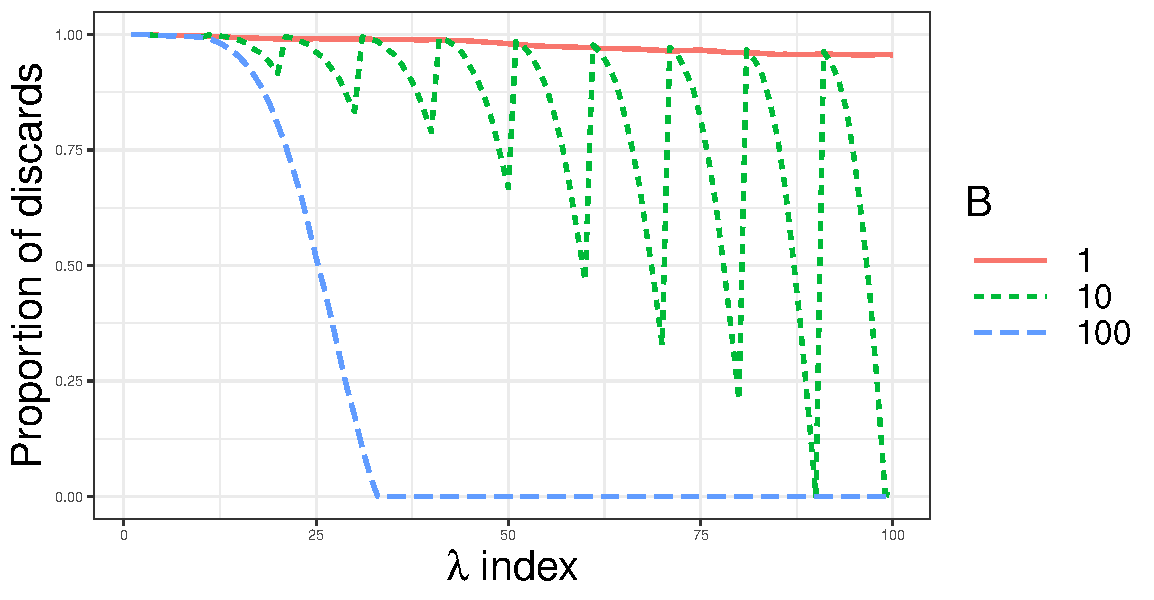
\includegraphics[scale = 0.6]{plots/batchsizes.pdf}    \caption{Proportion of features rejected by screening rules vs index of $\lambda$-values for different update delay.}
    \label{fig:3.4.1}
\end{figure}

BEDPP (Basic EDPP) rule is the special case of adaptive EDPP that never updates ($B=K$). When the reference does not get updated for a long time, the safe rule screening will eventually fail to discard any features and make the KKT condition checking cost increase to its maximum $np$. SEDPP rule is the special case that updates at every $\lambda$ value ($B=1$). It remains very powerful along the path, making the KKT condition checking cost small, but the safe screening itself is costly and takes $np$ time per $\lambda$-value. Adaptive EDPP can strike a balance between BEDPP and SEDPP. In this example, simply using fixed update period $B=10$ can reduce the safe screening cost by 90\% compared to SEDPP and reduce the KKT checking cost by 50\% to more than 90\% compared BEDPP.

This example also shows the timing of updates should be decided carefully and adaptively. For the first 10 $\lambda$-values, the safe rule stays powerful, which means the old reference is still exploitable. We may want delay the update to reduce average safe screening cost without harming the KKT condition checking cost much. For the last 20 $\lambda$-values however, the screening power drops to 0 quickly, which means the reference becomes useless quickly. Updating more frequently can greatly reduce the KKT condition checking cost with relatively small increase in safe screening cost. Moreover, the performance of adaptive EDPP rule also depends on many factors such as the data, the range of $\lambda$-values and spacing between $\lambda$-values. These suggest that simple updating rules like periodic updating cannot not be consistently efficient and we want a method that can automatically determine whether to update given current performance.

\subsubsection{Efficient updating algorithm}

From previous example, we assume the average cost is a convex function of distance from last update $B$, which decreases first and then after some optimal value increases again. If we want to minimize the average cost per $\lambda$-value, we need to update when using the old reference for one more $\lambda$-value will increase the average cost. That is, we should update the reference to $\lambda_{k+B}$ when $\bar{T}_k(B+1)>\bar{T}_k(B)$. For practice, we will update the reference to $\lambda_{k+B}$ when $\bar{T}_k(B)>\bar{T}_k(B-1)$ instead, because $\bar{T}_k(B+1)$ cannot be calculated without doing screening at $\lambda_{k+B+1}$. These two conditions should be close and thus this substitution should also be close to optimal. Combined with \eqref{eq:cost}, the latter condition will approximately be:

\begin{equation}
    \label{eq:crit}
    (B-1)|\mathcal{S}_{k+B}|-\sum_{b=1}^{B-1}|\mathcal{S}_{k+b}|>p.
\end{equation}


This updating condition is a greedy condition that only considers the cost up to the current $\lambda$ value. In practice, we cannot know about future $\lambda$ values so this is the most reasonable condition. In fact, it provides a robust strategy towards three most common scenarios. First, if the screening power stays high, meaning $\mathcal{S}_{k+b}$ is small for all $b$, then the left-hand-side of \eqref{eq:crit} will be small and thus at this point we will not update to further exploit the last update. Second, if the screening power has been high for a while but dropped suddenly, meaning $\mathcal{S}_{k+B}$ is large but $\mathcal{S}_{k+b}$ are mostly small for $b=1,2,...,B-1$, then the left-hand-side of \eqref{eq:crit} will be large and we will update the useless old reference to a new helpful one. Last, if the screening power drops dramatically right after the last update, meaning $\mathcal{S}_{k+b}$ are close to $p$ for $b=2,3,...,B$, then the left-hand-side of \eqref{eq:crit} will be approximately $p-|\mathcal{S}_1|<p$. We will not update although old reference is useless, because if we did, the new update would become useless quickly as well.

This adaptive updating condition fills in the condition on line 11 in Algorithm 1 and forms a complete pathwise lasso algorithm with adaptive hybrid screening. 


\section{Extension to other lasso type problems}
\label{sec:4}

The structure of the adaptive hybrid rule is easily extendable to any lasso problems that have corresponding sequential strong rule and sequential safe rule. After an adaptive safe rule is built, we can automatically apply the adaptive strong rule and the adaptive update algorithm to form a pathwise algorithm with adaptive hybrid screening. We are going to derive the extensions to two lasso type problems and show these extensions improve computation efficiency.

\subsection{Adaptive safe rule for sparse logistic regression}

The sparse logistic regression model can be defined as:

\begin{equation}
    \label{eq:logis}
    \hat{\beta}(\lambda)=\underset{(\beta,\beta_0)\in \mathbb{R}^p\times\mathbb{R}^1}{\mathrm{argmin}}-\frac{1}{n}\sum_{i=1}^n\{y_i\log\pi_i(\beta)+(1-y_i)\log(1-\pi_i(\beta))\}+\lambda||\beta||_1,
\end{equation}
where $\pi(\beta)=\{\pi_i(\beta)\}_{i=1}^n=\{p(y_i=1|x_{i1},x_{i2},...,x_{ip})\}_{i=1}^n=\{e^{\eta_i(\beta)}/(1+e^{\eta_i(\beta)})\}_{i=1}^n$ is the predicted value vector and $\eta(\beta)=X\beta+\beta_0\mathbf{1}$ is the linear function. $X$ are still the $n\times p$ standardized feature matrix but in this model the $y\in\{0,1\}^n$ is an unstandardized binary response vector. $\beta$ is still the $p\times1$ coefficient vector but we also need a $\beta_0$ as the intercept.

We can use SSR to do the strong rule screening with a small change according to the KKT condition. The residual vector now is $r(\lambda_k)=y-\pi(\hat{\beta}(\lambda_k))$. Then the SSR discards the $j$-th feature at $\lambda_{k+1}$ if \eqref{eq:ssr} holds.

For safe rule screening, instead of EDPP rules, Slores (sparse logistic regression screening rule)\citep{wang2014safe} is used. It was proposed as a one-step rule but it can be extended as a sequential rule with some minimal change and thus can be extended as adaptive rule. Let $\Tilde{y}=2y-1\in\{-1,1\}^n$, $r(\lambda_k)=y-\pi(\hat{\beta}(\lambda_k))$.

\begin{theorem}[Adaptive Slores]
For the sparse logistic regression model \eqref{eq:logis}, let $\lambda_0:=\max_j|x_j^Ty/n|$, $\Tilde{y}=2y-1\in\{-1,1\}^n$. Suppose we have a sequence of $\lambda$ values $\lambda_0>\lambda_1>...>\lambda_K$. $\forall\theta\in(0,1)^n$, let 

\begin{equation}
    \begin{split}
        g(\theta)&=\frac{1}{n}\sum_{i=1}^n\{\theta_i\log \theta_i+(1-\theta_i)\log(1-\theta_i)\},\\
    \nabla g_i(\theta) &= \frac{1}{n}\log\frac{\theta_i}{1-\theta_i}.
    \end{split}
\end{equation}

Under condition \eqref{eq:std} except for standardization for $y$, for any $k=1,2,...,K-1$, assume $\hat{\beta}(\lambda_k)$, $r(\lambda_k)=y-\pi(\hat{\beta}(\lambda_k))$, $x_*\in\{x_j:\hat{\beta}_j(\lambda_k)\neq0\} $, $\theta(\lambda_k)=\{r_i(\lambda_k)\Tilde{y}_i\}_{i=1}^n$ and $\hat{y}(\lambda_k):=\pi(\hat{\beta}(\lambda_k))$ are known. For any $k+b>k$, let

\begin{equation}
    R(\lambda_{k+b})=\sqrt{\frac{n}{2}\bigg[g\bigg(\frac{\lambda_{k+b}}{\lambda_k}\theta(\lambda_k)\bigg)-g\bigg(\theta(\lambda_k)\bigg)+\bigg(1-\frac{\lambda_{k+b}}{\lambda_k}\bigg)\bigg(\nabla g\big(\theta(\lambda_k)\big)\bigg)^T\theta(\lambda_k)\bigg]},
\end{equation}

$d(\lambda_{k+b})=\sqrt{n}(\lambda_k-\lambda_{k+b})/R(\lambda_{k+b})$. For $\xi = -1,1$ and $j=1,2,...,p$,

\begin{enumerate}
    \item If $-\xi sign(x_*^Ty)x_j^Tx_*\geq nd(\lambda_{k+b})$, then
    
    \begin{equation}
        T_\xi(\lambda_{k+b},x_j;r(\lambda_k))=\sqrt{n}R(\lambda_{k+b})-\xi x_j^Tr(\lambda_k);
    \end{equation}
    
    \item If $-\xi sign(x_*^Ty)x_j^Tx_*< nd(\lambda_{k+b})$, then
    
    \begin{equation}
        T_\xi(\lambda_{k+b},x_j;r(\lambda_k))=R(\lambda_{k+b})\sqrt{n+nu_\xi^2-2\xi u_\xi sign(x_*^Ty)x_j^Tx_*}-nu_\xi(\lambda_k-\lambda_{k+b})-\xi x_j^Tr(\lambda_k),
    \end{equation}
    where
    \begin{align}
        u_\xi&=\frac{-\xi a_1+\sqrt{\Delta}}{2a_2},\\
        a_0&=(x_j^Tx_*)^2-n^2d^2(\lambda_{k+b}),\nonumber\\
        a_1&=-2n\,sign(x_*^Ty)x_j^Tx_*\big(1-d^2(\lambda_{k+b})\big),\nonumber\\
        a_2&=n^2\big(1-d^2(\lambda_{k+b})\big),\nonumber\\
        \Delta&=a_1^2-4a_0a_1.\nonumber
    \end{align}
\end{enumerate}

Then $\hat{\beta}_j(\lambda_{k+b})=0$ if
        \begin{equation}
            \max_{\xi=\pm1} T_\xi(\lambda_{k+b},x_j;r(\lambda_k))
        \end{equation}
\end{theorem}

When computing the adaptive Slores, $\{x_j^Ty\}_{j=1}^p$ needs to be computed only once, stored and reused for the whole solution path. $\{x_j^Tx_*\}_{j=1}^p$ can be reused unless $x_*$ changes. Other than those two terms, the only term that requires expensive $O(np)$ computation is $\{x_j^Tr(\lambda_k)\}_{j=1}^p$, which only needs to be computed at the time of each update. Thus algorithm 1 for adaptive hybrid rule can be done with Slores rule instead of EDPP rule to form Ada-SSR-Slores that does screening for sparse logistic regression model.

\subsection{Adaptive safe rule for group lasso}

The group lasso problem \citep{yuan2006model} can be defined as:

\begin{equation}
    \label{eq:glasso}
    \hat{\beta}(\lambda) = \underset{\beta\in \mathbb{R}^p}{\mathrm{argmin}}\frac{1}{2n}\bigg|\bigg|y-\sum_{g=1}^GX_g\beta_g\bigg|\bigg|_2^2+\lambda\sum_{g=1}^G\sqrt{p_g}||\beta_g||_2,
\end{equation}
where $\beta=(\beta_1^T,...,\beta_G^T)^T$, $X_g$ is a $n\times p_g$ sub-matrix consisting of columns of $X$ corresponding to features in group $g$, $g=1,2,...,G$. Besides standardization in \eqref{eq:std}, we apply an addition level of standardization at the group level\citep{breheny2015group}:

\begin{equation}
    \label{eq:stdg}
    X_g^TX_g=nI_{p_g\times p_g},\qquad g=1,2,...,G.
\end{equation}

According to the KKT condition, we can use SSR to do strong rule screening. Given $r(\lambda_k)=y-\sum_{g=1}^GX_g\hat{\beta}_g(\lambda_k)$, we discard features in the $g$-th group at $\lambda_{k+1}$ if:

\begin{equation}
    \bigg|\bigg|\frac{1}{n}X_g^Tr(\lambda_k)\bigg|\bigg|_2<\sqrt{p_g}(2\lambda_{k+1}-\lambda_k).
\end{equation}

For safe rule screening, we have SEDPP for group lasso\citep{wang2013lasso} and we can extend it the adaptive EDPP rule for group lasso.

\begin{theorem}[Adaptive EDPP for group lasso]
For the group lasso problem \eqref{eq:glasso}, let $\lambda_0:=\max_j\frac{||X_g^Ty||_2}{n\sqrt{p_g}}$. Suppose we have a sequence of $\lambda$ values $\lambda_0>\lambda_1>...>\lambda_K$. Under condition \eqref{eq:std} and \eqref{eq:stdg}
    \begin{enumerate}
        \item For any $k=1,2,...,K-1$, given $\hat{\beta}(\lambda_k)$, $r(\lambda_k)$ and $\hat{y}(\lambda_k):=\sum_{g=1}^GX_g\hat{\beta}_g(\lambda_k)$, then for any  $k+b>k$, $\hat{\beta}_g(\lambda_{k+b})=0$ if
        \begin{equation}
            \begin{split}
                &\left|\left|2\lambda_{k+b}X_g^Tr(\lambda_k)+(\lambda_k-\lambda_{k+b})\left( X_g^Ty-\frac{y^T\hat{y}(\lambda_k)X_g^T\hat{y}(\lambda_k)}{||\hat{y}(\lambda_k)||_2^2}\right)\right|\right|_2\\
                &<2n\lambda_k\lambda_{k+b}\sqrt{p_g}-(\lambda_k-\lambda_{k+b})\sqrt{n||y||_2^2-\frac{n(y^T\hat{y}(\lambda_k))^2}{||\hat{y}(\lambda_k)||_2^2}}
            \end{split}
        \end{equation}
        \item For k=0, i.e., $\lambda_k=\lambda_0$, let $X_*=argmax_{X_g}\frac{||X_g^Ty||_2}{n\sqrt{p_g}}$ with dimension $n\times p_*$, then for any $b>0$, $\hat{\beta}_g(\lambda_{k+b})=0$ if
        \begin{equation}
        \left|\left|(\lambda_0+\lambda_b)X_g^Ty-(\lambda_0-\lambda_b)X_g^TX_*X_*^Ty\right|\right|_2<2n\lambda_0\lambda_b\sqrt{p_g}-(\lambda_0-\lambda_b)\sqrt{n||y||_2^2-n^2\lambda_0^2p_*}.
    \end{equation}
    \end{enumerate}
\end{theorem}

Similar to Adaptive EDPP rule, three expensive computations are $\{X_g^Ty\}_{g=1}^G$, $\{X_g^TX_*\}_{g=1}^G$ and $\{X_g^Tr(\lambda_k)\}_{g=1}^G$. The first and second only need to be computed once for the whole solution path. The last only needs to be computed at the time of each update with cost $O(np)$. The adaptive EDPP for group lasso, combined with the previous SSR, forms the Ada-SSR-EDPP for group lasso.

\section{Experiments}
\label{sec:5}

In this section conduct experiments solving lasso model on both simulated data sets and real data sets, to show our proposed adaptive hybrid rule screening method outperforms previous screening method such as SSR, SEDPP, HSSR and Slores. Active-set cycling in \ref{sec:active} is always used with all screening methods because it can be easily combined with any screening methods with no extra cost.

The adaptive hybrid rule screening is implemented in the \textbf{R} package \textbf{biglasso} and we will use this package for our experiment. Compared to traditional packages that solve lasso problem, such as \textbf{glmnet}, \textbf{biglasso} focuses on efficiently solving lasso problem with high-dimensional data sets that have a large number of features. First, it utilized the memory-mapping techniques that stores the data set on the disk and reads in only the part of the data necessary for model solving. Second, it applied screening rules to reduce both the computation cost and memory cost as we have discussed. These two features together help \textbf{biglasso} to outperform other packages. We will show that our new screening method will result in a new version of the package that shows significant improvement compared to previous version. 

For all the following experiments, we will solve the lasso model along a path of $100$ $\lambda$-values with the maximum $\lambda_0=\max_j|x_j^Ty/n|$ determined by the data, the minimum $\lambda_K=0.05\lambda_0$ and the rest $\lambda$-values equally spaced between on log scale.

\subsection{Simulation study}
\label{sec:sim}

\subsubsection{Lasso model}

In this part, we will solve the standard lasso problem \eqref{eq:lasso} with different screening methods: Active-set Cycling (AC) alone, SSR, SEDPP, HSSR and adaptive hybrid rule (AHR). The AHR is Ada-SSR-EDPP which uses EDPP as the safe rule. Note that AC is always incorporated with all other screening rules, so using AC alone can be considered as a baseline for this comparison.

The data will be simulated from the model: $y=X\beta+0.1\epsilon$. $X$ and $\epsilon$ are sampled i.i.d from $N(0,1)$. $\beta$ will have $s$ randomly selected elements equally spaced between $[-\beta_{max},\beta_{max}]$ and the rest $p-s$ elements are zeros. The lasso model is solved along a grid of $L$ $\lambda$-values equally spaced on the log scale between $[\lambda_{\max},\lambda_{\min}]$. Each setting is replicated $10$ times to calculate the average time cost. By default we set $p=10,000$, $n=1,000$, $s=20$, $\beta_{max}=1$, $L=100$, $\lambda_{\min}/\lambda_{\max}=0.05$. We consider the following cases where one of the variables above is varying at a time:

\begin{enumerate}
    \item \textbf{Varying number of features:} $p$ from $1,000$ to $100,000$.
    \item \textbf{Varying sample size:} $n$ from $200$ to $10,000$.
    \item \textbf{Varying signal strength:} $\beta_{max}$ from $0.05$ to $1$.
    \item \textbf{Varying sparsity:} $s$ from $10$ to $300$ while controlling total signal size $\beta_{max}\times s=20$.
    \item \textbf{Varying number of grid points:}  $L$ from $20$ to $1000$.
    \item \textbf{Varying range of grid:}  $\lambda_{\min}/\lambda_{\max}$ from $0.5$ to $0.002$.
    \item \textbf{Varying number of grid points $L$ with fixed spacing:} $L$ from $20$ to $1000$ while controlling $\lambda_{\min}/\lambda_{\max}$ so that the spacing of the $\lambda$-values on the log scale is the same.
\end{enumerate}

\begin{figure}[h]
    \centering
    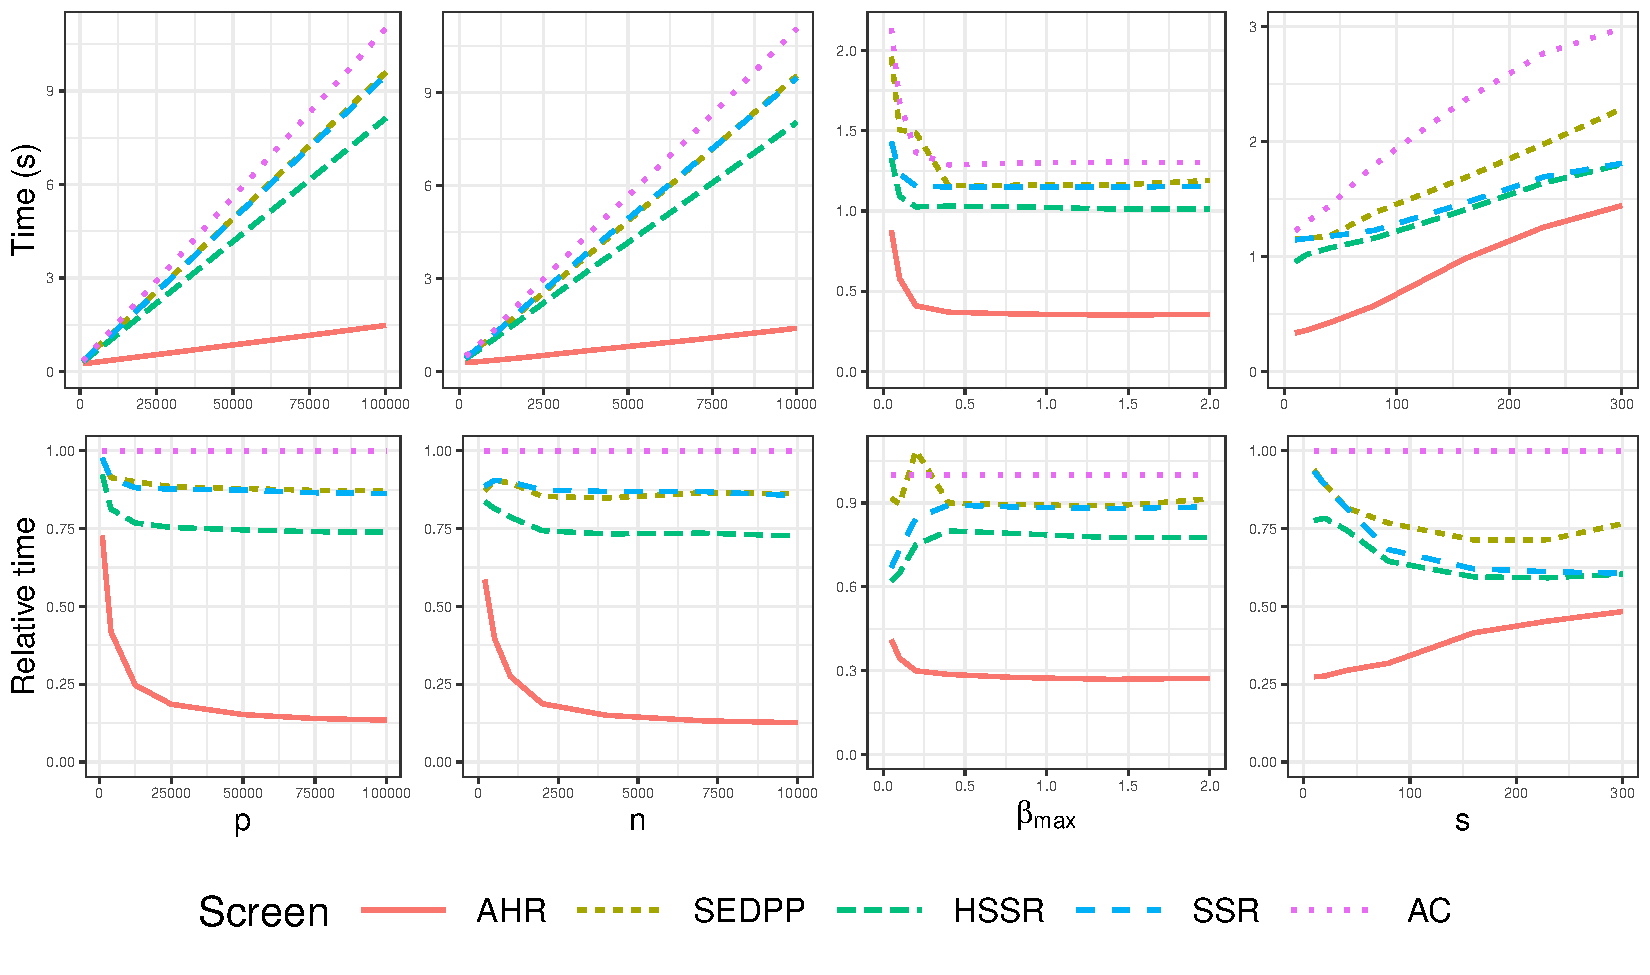
\includegraphics[scale = 0.59]{plots/511.pdf}    \caption{Comparing speed of screening methods for lasso model under different settings. Top row: computation time in second. Bottom row: relative computation time compared to AC. First column: varying number of features $p$. Second column: varying sample size $n$. Third column: varying signal strength $\beta_{max}$. Fourth column: varying sparsity $s$.}
    \label{fig:5.1.1a}
\end{figure}

\begin{figure}[h]
    \centering
    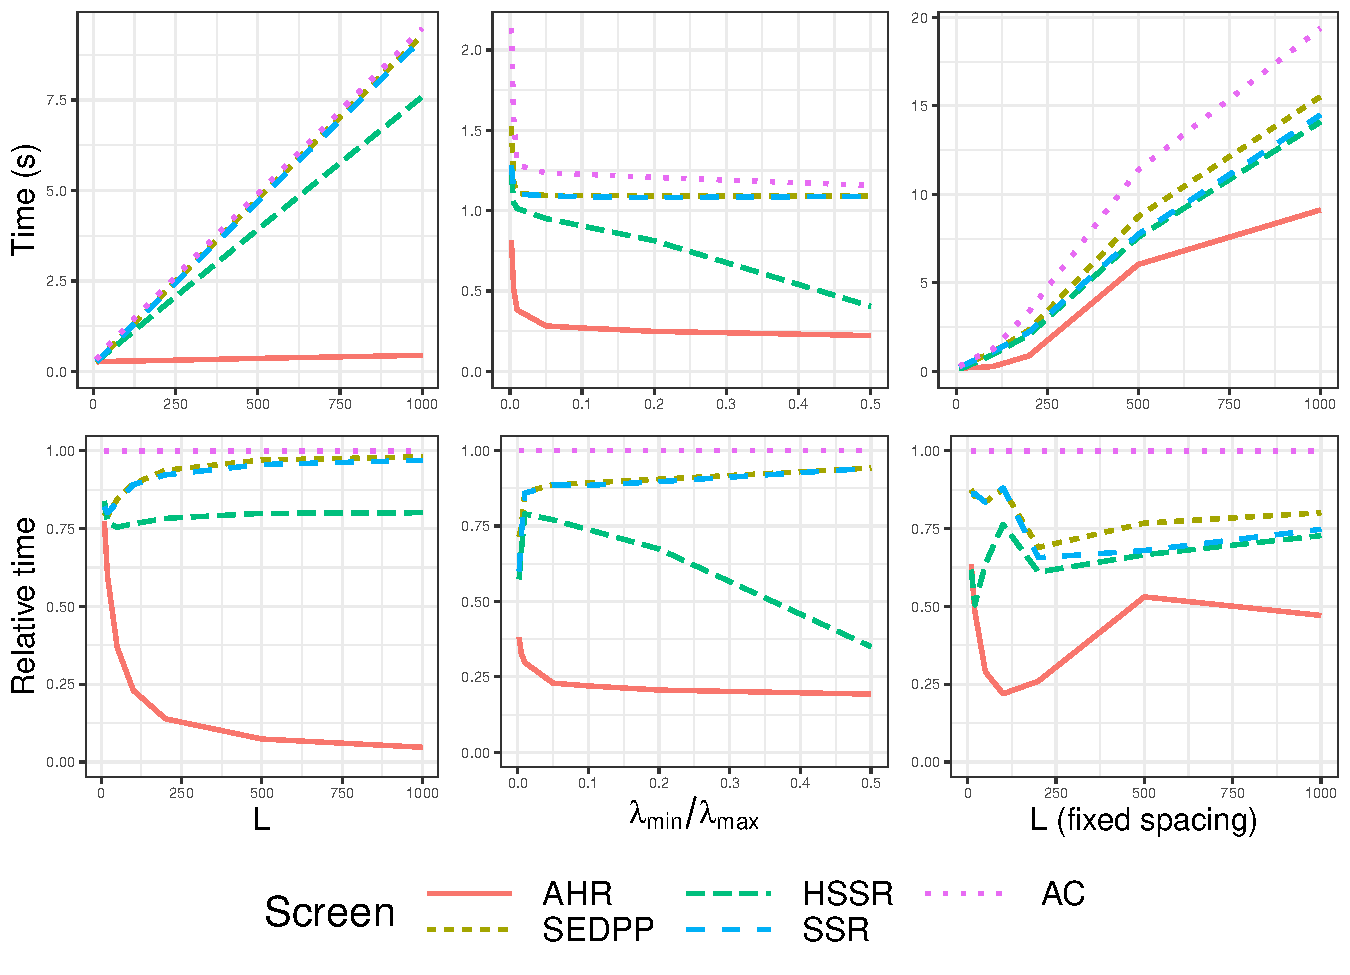
\includegraphics[scale = 0.59]{plots/511b.pdf}    \caption{Comparing speed of screening methods for lasso model under different settings. Top row: computation time in second. Bottom row: relative computation time compared to AC. First column: Varying number of grid points $L$. Second column: Varying range of grid $\lambda_{\min}/\lambda_{\max}$. Third column: Varying number of grid points $L$ with fixed spacing.}
    \label{fig:5.1.1b}
\end{figure}

Figure 2 and Figure 3 shows the computation time (top row) and relative computation time compared to AC (bottom row) of solving lasso problem with different screening methods. The AHR is uniformly the fastest under all settings. Most of the time it is 2-8 times faster than any other screening methods. It outperforms other methods especially when the data set is large (large $n$ or large $p$), the active features are sparse among all features (small $s$) or the grid of $\lambda$-value is fine (large $L$ or $\lambda_{\min}/\lambda_{\max}$). 

There are several atypical cases when AHR's advantage over other methods is not as significant: (1) $p$ or $n$ is small. This corresponds a small data set and computation will be less challenging. (2) $\beta_{max}$ is close to zero. This means all the nonzero coefficients are close to zero and are hard to be distinguished from zero coefficients. This can cause problem for any statistical learning methods. (3) $s$ is large. In this case, the underlying model that generate the data set is not sparse in the sense that proportion of nonzero coefficients is not small. Lasso model would not be the optimal model to analyse such an data set. (4) $L$ is small. In this case, only a coarse grid of $\lambda$-values are considered. The $\lambda$-value selected in this case may be far from optimal.

We also tried varying other factors, for example, varying the correlation among features in $X$, varying the sparsity with fixed signal strength or varying the minimum $\lambda$-value $\lambda_K$. The AHR also shows uniform advantage over other method when those factors vary in reasonable ranges.

\subsubsection{Sparse logistic regression model}

In this part, we will replicate the previous experiment, expect that now we will solve the sparse logistic regression model with the following screening methods: SSR, HSSR with Slores as the safe rule (HSlores), and the adaptive method Ada-SSR-Slores with Slores as the safe rule (ASlores). SSR is implemented in all of the three screening methods so it will be considered as the baseline.

The data will be simulated from the model: $y=\mathbf{1}\{X\beta+0.1\epsilon >0\}$. $X$ and $\epsilon$ are sampled i.i.d from $N(0,1)$. $\beta$ will have $s$ randomly selected elements equally spaced between $[-\beta_{max},\beta_{max}]$ and the rest $p-s$ elements are zeros. Each setting is replicated $10$ times to calculate the average time cost. We consider the same 7 cases we have considered in the previous experiment.

\begin{figure}[h]
    \centering
    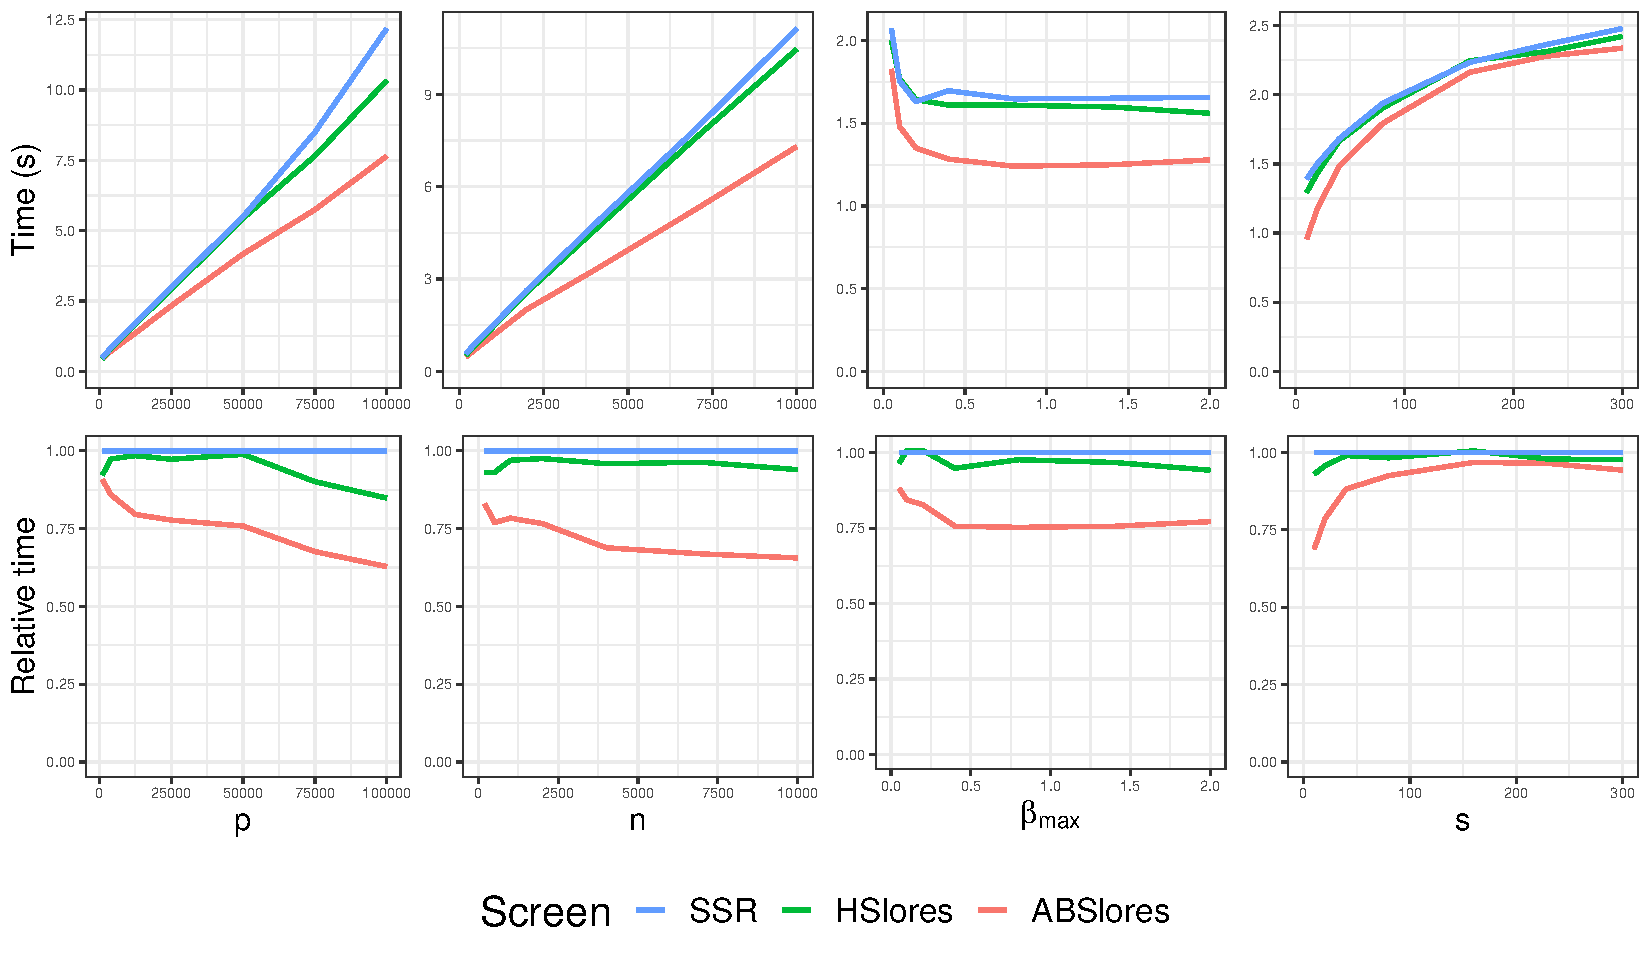
\includegraphics[scale = 0.59]{plots/512.pdf}    \caption{Comparing speed of screening methods for sparse logistic regression model under different settings. Top row: computation time in second. Bottom row: relative computation time compared to SSR. First column: varying number of features $p$. Second column: varying sample size $n$. Third column: varying signal strength $\beta_{max}$. Fourth column: varying sparsity $s$.}
    \label{fig:5.1.2a}
\end{figure}

\begin{figure}[h]
    \centering
    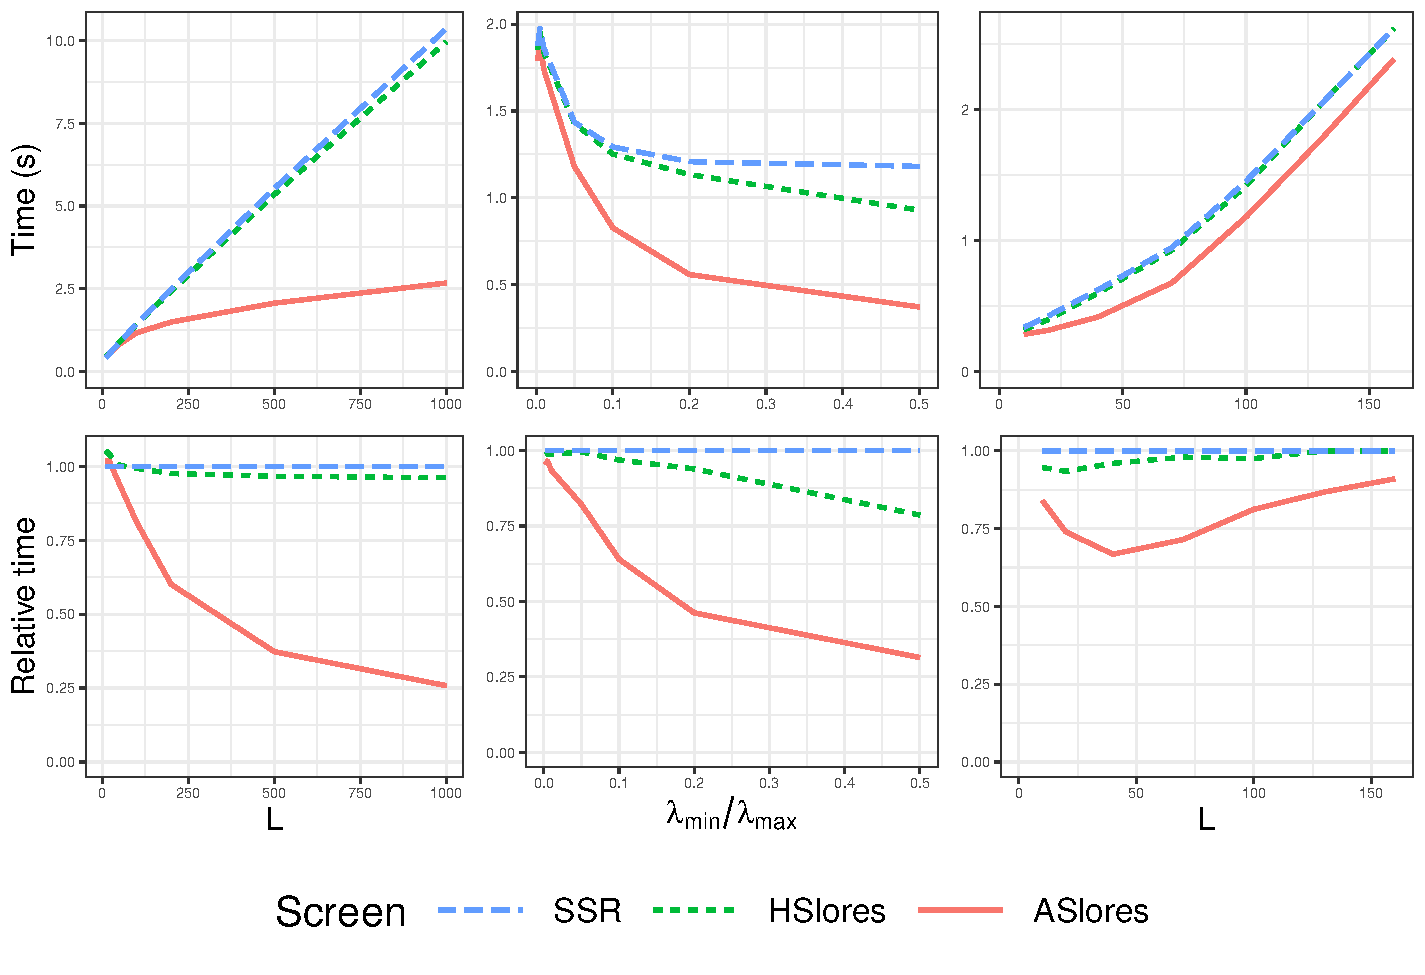
\includegraphics[scale = 0.59]{plots/512b.pdf}    \caption{Comparing speed of screening methods for sparse logistic regression model under different settings. Top row: computation time in second. Bottom row: relative computation time compared to SSR. First column: Varying number of grid points $L$. Second column: Varying range of grid $\lambda_{\min}/\lambda_{\max}$. Third column: Varying number of grid points $L$ with fixed spacing.}
    \label{fig:5.1.2b}
\end{figure}

Figure 4 and 5 show the computation time (top row) and relative computation time compared to SSR (bottom row) of solving sparse logistic regression problem with different screening methods. ASlores is also uniformly faster than other methods and this improvement is significant except for some atypical cases motioned before.


\subsection{Real data analysis}
\label{sec:real-data}

In previous sections, we used simulation to compare the screening methods under different scenario. In real world, data may be generated from different complicated models that cannot be covered by a simulation study, so in this section we are going to test the screening methods for lasso model on some real data sets to make sure our comparison conclusion is representative in real world. Following the studies of \citep{wang2013lasso, xiang2016screening, Zeng2021}, we will test the lasso screening methods on the following data sets:

\begin{enumerate}
    \item \textbf{Breast cancer gene expression data
(GENE):} this data has expression measurements of $p=17,322$ genes from $n=536$ patients. The response is the expression measurement of the gene BRCA1, which has been identified to be related to risk of breast cancer.
    \item \textbf{MNIST handwritten image data
(MNIST):} this data set has $60,000$ images in the training set and $10,000$ images in the testing set. Each image is a $28\times 28=784$ pixels image of handwritten digits. We use the training set to form a $n=784\times p=60,000$ feature matrix, treating pixels as samples and images as features. Then an image from the testing set is randomly selected as the response.
    \item \textbf{ Cardiac fibrosis genome-wide association data
(GWAS):} this data set has $p=660,496$ single nucleotide
polymorphisms (SNPs) collected from $n=313$ human hearts. The response is the log of the ratio of cardiomyocytes to fibroblasts in the heart tissue, which is associated with heart failure.
    \item \textbf{Subset of New York Times bag-of-words data
(NYT):} the raw data set is a $300,000\times 102,660$ matrix, each row being a document and each column being number of occurrence of a specific word in those documents. We selected $n=5,500$ documents by removing documents with low word counts. Then $55,000$ words are selected as the features and a randomly selected word is the response.

\end{enumerate}


For 1 and 3, we replicate the experiment 10 times to take the average. For 2 and 4, since in each experiment the response is randomly selected, we replicate the experiment 50 times to get an accurate estimate. Table 1 compares the average computation time for different screening methods in these data sets.

\begin{table}[H]
\centering
\begin{tabular}{l|l|l|l|l}
\hline
 & GENE & MNIST & GWAS & NYT \\
Screening method & n=536 & n=784 & n=313 & n=5,500 \\
 & p=17,322 & p=60,000 & p=660,496 & p=55,000 \\ \hline
AC & 2.14 (0.03) & 6.82 (0.07) & 46.67 (0.13) & 59.20 (1.89) \\
SSR & 1.34 (0.01) & 5.20 (0.01) & 25.34 (0.08) & 35.40 (0.44) \\
SEDPP & 1.38 (0.01) & 8.40 (0.45) & 25.48 (0.05) & 53.69 (3.81) \\
HSSR & 1.21 (0.01) & 3.44 (0.07) & 23.85 (0.06) & 31.05 (0.80) \\
AHR & \textbf{0.71 (0.01)} & \textbf{1.15 (0.02)} & \textbf{8.80 (0.03)} & \textbf{12.71 (1.05)} \\\hline
\end{tabular}
\caption{Average computing time in second (standard error) for solving the lasso model}
\end{table}

AHR again outperforms other screening methods on all data sets, faster than the fastest of the rest by 70\% to 200\%. Also note that the performance of SEDPP varies a lot in MNIST and NYT data sets, where the response is randomly selected in each replication, suggesting that the speed of SEDPP is sensitive to the data. AHR is built with SEDPP as the safe rule but does not have the problem of instability, because it can adaptively adjust itself according the performance of the safe rule.



\subsection{Big data performance}

Ultra high dimensional big data that is too large to be fit into the memory is the real challenge and is the place where the help of a good screening method is wanted most. We test the screening methods on a data from a genome-wide association study on 1,080 subjects with heart conditions. We want to identify genetic factors that are associated with some heart condition severity measurements. After imputing and filtering, there are $p=11,830,470$ SNP measurements used as the features. The size of the file storing the feature matrix is 96G and we conduct the test on a machine with 32G RAM. We choose a larger $\lambda_{\min} =0.5\lambda_{\max}$ to avoid having more features selected than the number of observations, where the solution becomes not unique.

For the lasso model, we choose the Left ventricular ejection fraction (LVEF) as the response. It measures the proportion of blood being pumped out of the left ventricle of the heart (the main pumping chamber) with each contraction. Lower value means severer heart failure. $n=973$ out of 1,080 subjects have this measurement and they will be considered as the sample for this analysis. The experiment is replicated 5 times to take the average, shown in the Table 2.

\begin{table}[H]
\centering
\begin{tabular}{l|l|l|l|l|l}
\hline

Screening method & AC\,\,\,\,\,\,\,\,\,    & SSR\,\,\,\,\,\,   & SEDPP & HSSR\,\,\,  & AHR\,\,\,\,\,\,  \\
\hline
Time & 183.6 & 78.6 & 78.6 & 84.9 & 13.6\\
Standard error & 0.43 & 0.65 & 0.20 & 0.48 & 0.15
 \\\hline
\end{tabular}
\caption{Average computing time in minute and standard error for solving the lasso model on big data}
\end{table}

For the sparse logistic model, we choose the New York Heart Association (NYHA) Functional Classification as the response. It classifies patients by how much they are limited during physical activity. The classes range from 1 to 4 so we combine class 1 and 2 as the negative class with no or slight limitation of physical activity and class 3 and 4 as the positive class with substantial limitation. $n=1008$ out of 1,080 subjects have this measurement and they will be considered as the sample for this analysis. The experiment is replicated 5 times to take the average, shown in the Table 3.

\begin{table}[H]
\centering
\begin{tabular}{l|l|l|l}
\hline

Screening method & SSR\,\,\,\,\,\,\,\,\,    & HSlores\,\,\,\,\,\,   & ASlores   \\
\hline
Time & 82.7 & 107.5 & 51.7 \\
Standard error & 0.10 & 0.67 & 0.17 
 \\\hline
\end{tabular}
\caption{Average computing time in minute and standard error for solving the sparse logistic model on big data}
\end{table}

For both the lasso model and the sparse logistic model, the purposed adaptive hybrid methods outperforms other methods with great reduction in computation time. On the lasso model, the adaptive hybrid method achieves 6 times speedup.

\section{Conclusion}
\label{sec:6}

In this paper, we proposed the novel adaptive hybrid screening framework for efficient lasso type problem optimization over the solution path. The key idea is cleverly reusing the reference for screening along the path until updating to a new reference is beneficial for computation cost.  We developed three instances in this framework: Ada-SSR-EDPP, Ada-SSR-Slores and Ada-SSR EDPP for group lasso, for 3 different types of lasso problems. We tested the first two in extensive numeric experiments on both simulated data and real data, including a ultra big data that does not fit into the memory. Our proposed rules outperformed other state-of-the-art screening methods uniformly, especially in the most challenging scenarios. 

Ada-SSR-EDPP and Ada-SSR-Slores have been implemented in  publicly accessible \textbf{R} packages \textbf{biglasso}\citep{zeng2017biglasso}, which was used to carry out the numeric experiments.

Our adaptive hybrid screening framework also has great flexibility for extensions. It can substitute coordinate descent with any other faster lasso problem optimizer, SSR with any other stronger strong rules and the adaptive updating algorithm with any other cleverer algorithm. Most importantly, most sequential safe rules can be modified as adaptive safe rules and fit into our framework. This lead to several future extensions. First, if a stronger safe rule is developed, our framework can better exploit its power and lead to an even faster algorithm. Second, there are still many lasso type problems that do not have corresponding sequential safe rules, such as sparse Cox regression, sparse Poisson regression and sparse SVM. Once they are developed, they can be fit into our framework to produce efficient algorithm for other types of lasso problem.





\bibliography{ref}

\end{document}
